% FONTE TEMA https://github.com/matze/mtheme
\documentclass[aspectratio=1610]{beamer}
%\documentclass[aspectratio=1610, handout]{beamer}
\usepackage[utf8]{inputenc}
\usepackage{ragged2e}
\usepackage{xcolor}
\usepackage[italian]{babel}
\usepackage{multirow}
\usepackage{silence}
\WarningFilter{beamer}{}
\WarningFilter{metropolis}{}
\usetheme[progressbar=frametitle,titleformat=smallcaps]{metropolis}
\setbeamertemplate{frame numbering}[fraction]
\setbeamercovered{dynamic}
\definecolor{rosso}{RGB}{255, 0, 0}
\definecolor{giallo}{RGB}{254,212,23}
\hypersetup{colorlinks=true,linkcolor=black,urlcolor=rosso}
\setbeamercolor{palette primary}{fg=black, bg=giallo}
\setbeamercolor{background canvas}{bg=white}
\setbeamercolor{normal text}{fg=black}
\setbeamercolor{progress bar}{fg=rosso}
\setbeamercolor{framesubtitle}{fg=rosso}
\setbeamercolor{normal text .dimmed}{fg=giallo}
\setbeamercolor{block title alerted}{fg=rosso, bg=giallo}
\setbeamerfont{caption}{size=\tiny}
\setbeamerfont{caption name}{size=\tiny}
\setlength{\abovecaptionskip}{0pt}
\makeatletter
\metroset{block=fill}
\setlength{\metropolis@progressinheadfoot@linewidth}{1pt} 
\setlength{\metropolis@progressonsectionpage@linewidth}{1pt}
\setlength{\metropolis@titleseparator@linewidth}{1pt}
\makeatother

\title{TUTORIAL APP INVENTOR}
\subtitle{Esercizi base per imparare a programmare con App Inventor}
\date{}
\institute{\textit{
        Fonti:
        \begin{itemize}
            \item[-] \href{https://appinventor.mit.edu/explore/ai2/tutorials}{App Inventor Tutorials}
            \item[-] \href{https://appinventor.mit.edu/explore/library}{App Inventor Learning Library}
            \item[-] \href{https://www.youtube.com/c/MITAppInventor123}{App Inventor YouTube Channel}
        \end{itemize}
    }
}

\begin{document}

\begin{frame}[plain, noframenumbering]
    \titlepage
\end{frame}

\begin{frame}{TUTORIAL APP INVENTOR}
    \begin{alertblock}{SITI DI RIFERIMENTO}
        \begin{minipage}{0.98\linewidth}
            \justifying
            \begin{itemize}
                \item \textbf{\href{https://appinventor.mit.edu/explore/ai2/tutorials}{App Inventor Tutorials}}: una sezione del sito ufficiale di App Inventor dedicata a 
                fornire guide passo-passo per iniziare a programmare con App Inventor, con esempi di progetti 
                e attività per principianti.
                \pause
                \item \textbf{\href{https://appinventor.mit.edu/explore/library}{App Inventor Learning Library}}: una raccolta di risorse, tutorial e progetti 
                creati dalla comunità di App Inventor per aiutare i principianti a imparare a programmare.
                \pause
                \item \textbf{\href{https://www.youtube.com/c/MITAppInventor123}{App Inventor YouTube Channel}}: il canale ufficiale di App Inventor su YouTube, 
                dove è possibile trovare tutorial video, dimostrazioni di progetti e aggiornamenti sulle nuove funzionalità di App Inventor.
            \end{itemize}
        \end{minipage}
    \end{alertblock}
\end{frame}

\section{ESERCIZI BASE}

\begin{frame}{ESERCIZIO 1: MAPPA}
    \begin{figure}
        \href{https://lelecazza.it/lezioni/programmazione_a_blocchi/materiale/lezioni/4_tutorial_app_inventor/video/esercizio1.mp4}{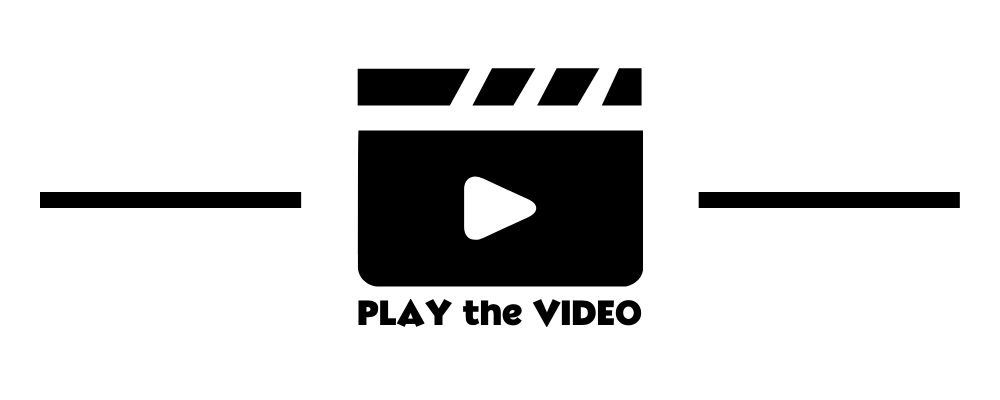
\includegraphics[width=\linewidth]{img/play.png}}
        \caption{{Scarica la \href{https://lelecazza.it/lezioni/programmazione_a_blocchi/materiale/lezioni/4_tutorial_app_inventor/soluzioni/esercizio1.aia}{soluzione}}}
    \end{figure}
\end{frame}

\begin{frame}{ESERCIZIO 1}
    \begin{alertblock}{MAPPA}
        \begin{minipage}{0.96\linewidth}
            \begin{itemize}
                \justifying
                \item Inserisci un blocco impaginazione di tipo ``DisposizioneOrizzontale'' e al suo interno 
                inserisci due blocchi ``Etichetta'' e due blocchi ``Pulsante'' (modificane nome e dimensione)
                \pause
                \item Inserisci un blocco Maps di tipo ``Mappa'' e posizionalo sotto il blocco di impaginazione (modificane nome e dimensione)
                \pause
                \item Inserisci un blocco di tipo ``Pulsante'' e posizionalo sotto il blocco Mappa (modificane nome e dimensione)
                \pause
                \item Crea tre variabili globali: una lista per contenere i ``Marker'' e due interi per latitudine e longitudine
            \end{itemize}
        \end{minipage}
    \end{alertblock}
\end{frame}

\begin{frame}{ESERCIZIO 1}
    \begin{alertblock}{MAPPA}
        \begin{minipage}{0.96\linewidth}
            \begin{itemize}
                \justifying
                \item Fai in modo che alla pressione del tasto di ricerca la mappa venga centrata sulla posizione 
                inserita nei campi di latitudine e longitudine
                \pause
                \item Fai in modo che alla pressione prolungata sulla mappa i valori di latitudine e longitudine vengano 
                inseriti nei campi di latitudine e longitudine
                \pause
                \item Fai in modo che alla pressione del tasto di salvataggio venga creato un marker (aggiungendolo alla lista dei ``Marker'') 
                nella posizione inserita nei campi di latitudine e longitudine.
            \end{itemize}
        \end{minipage}
    \end{alertblock}
\end{frame}

\begin{frame}{ESERCIZIO 2: PAINT}
    \begin{figure}
        \href{https://lelecazza.it/lezioni/programmazione_a_blocchi/materiale/lezioni/4_tutorial_app_inventor/video/esercizio2.mp4}{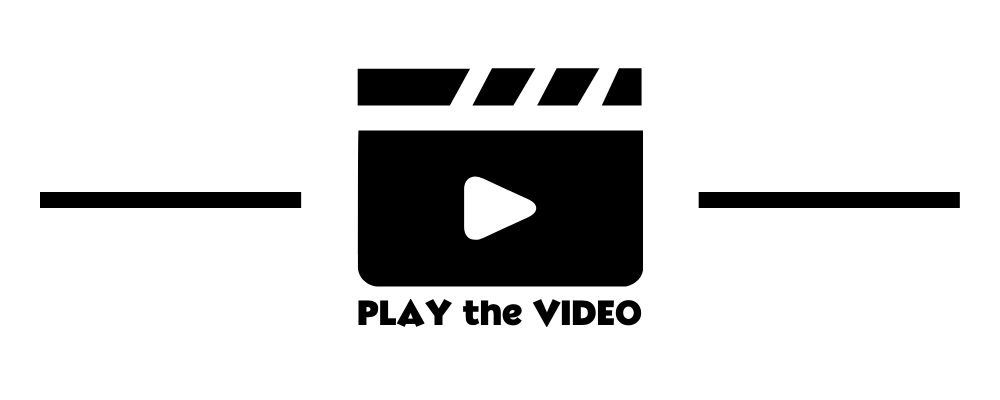
\includegraphics[width=\linewidth]{img/play.png}}
        \caption{{Scarica la \href{https://lelecazza.it/lezioni/programmazione_a_blocchi/materiale/lezioni/4_tutorial_app_inventor/soluzioni/esercizio2.aia}{soluzione}}}
    \end{figure}
\end{frame}

\begin{frame}{ESERCIZIO 2}
    \begin{alertblock}{PAINT}
        \begin{minipage}{0.96\linewidth}
            \begin{itemize}
                \justifying
                \item Inserisci un blocco impaginazione di tipo ``DisposizioneOrizzontale'' e al suo interno 
                inserisci un blocco ``SelettoreAScorrimento'' e un blocco ``Pulsante'' (modificane nome e dimensione)
                \pause
                \item Inserisci un blocco Disegno e Animazione di tipo ``Stage'' e posizionalo sotto il blocco di impaginazione (modificane nome e dimensione)
                \pause
                \item Fai in modo che al trascinamento del dito sullo stage venga disegnato un cerchio (con raggio 10) nella posizione 
                del trascinamento (X e Y attuali del trascinamento)
            \end{itemize}
        \end{minipage}
    \end{alertblock}
\end{frame}

\begin{frame}{ESERCIZIO 2}
    \begin{alertblock}{PAINT}
        \begin{minipage}{0.96\linewidth}
            \begin{itemize}
                \justifying
                \item Fai in modo che al tocco del selettore a scorrimento venga creata una lista di colori tra cui scegliere associando 
                ogni colore a un testo (es. rosso, verde, blu) che verrà mostrato nel selettore a scorrimento
                \pause
                \item Fai in modo che dopo la selezione del testo mostrato venga effettivamente cambiato il colore 
                impostato per il disegno dei cerchi nello stage (associando ogni testo al colore corrispondente)
                \pause
                \item Fai in modo che alla pressione del tasto di pulizia dello stage venga cancellato tutto ciò che è stato 
                disegnato nello stage e la selezione del colore venga resettata sul colore iniziale (nero).
            \end{itemize}
        \end{minipage}
    \end{alertblock}
\end{frame}

\end{document}